\documentclass[a4paper,12pt]{article}
\usepackage[utf8]{inputenc}
\usepackage[T1]{fontenc}
\usepackage[frenchb]{babel}
\frenchbsetup{StandardLists=true} 
\usepackage{hyperref}
\usepackage{multirow}
\usepackage{graphicx}
\usepackage{amsfonts}
\linespread{1.5}
\newcommand\tab[1][]{\hspace*{#1}}
\newcommand{\lt}{\ensuremath <}
\newcommand{\gt}{\ensuremath >}
\usepackage{amsmath}
\DeclareMathOperator{\arccot}{arccot}
\usepackage{xcolor}
\newcommand\Warning{%
 \makebox[1.4em][c]{%
 \makebox[0pt][c]{\raisebox{.1em}{\small!}}%
 \makebox[0pt][c]{\color{red}\Large$\bigtriangleup$}}}%
\setlength{\parindent}{0cm}

\begin{document}

%%---------------------------------------
%   FIRST PAGE                             
%%---------------------------------------

\begin{titlepage}
\begin{center}

\includegraphics[width=0.7\textwidth]{ephec.png}\\[0.5cm]

% Title
\rule{\linewidth}{0.2mm} \\[0.4cm]
{ \huge \bfseries Synthèse de mathématique \\[0.4cm] }
\rule{\linewidth}{0.2mm} 
\vfill

% Author and supervisor
\noindent
\begin{minipage}{0.4\textwidth}
  \begin{flushleft} \large
    \emph{Auteur :} Simon \textsc{Barré}\\
  \end{flushleft}
\end{minipage}
\vfill
\large
\today
\end{center}
\end{titlepage}
\renewcommand{\familydefault}{\sfdefault}

\newpage
\tableofcontents
\clearpage

\section*{Avant propos}
Synthèse réaliser depuis le syllabus du cours et mes notes personnels, des erreurs peuvent s'y êtres glissées, rester vigilant.

Le chapitre Numération à été volontairement ignorer, si vous avez le coeur de le synthétiser, je vous en prie.  

Équation écrite grâce à l'aide du site : \\ \tab[0.65cm]\url{http://visualmatheditor.equatheque.net/VisualMathEditor.html}

\section*{Répartition des points}
\begin{tabular}{lcc} 
    Trigonométrie & 15\% & \\ \hline
    Logique & 9\% &  \multirow{2}{*}{18\%} \\
    Numération & 9\% & \\ \hline
    Fonctions polynomiales & 7\% &  \multirow{2}{*}{20\%} \\
    Dérivation & 13\% &  \\ \hline
     Exponentiels et logarithmes & 11\% &  \multirow{2}{*}{22\%} \\
    Complexes & 11\% &  \\ \hline
    Intégration & 15\% &  \\ \hline
    Statistiques & 10\% & \\
\end{tabular}

\newpage
\section{Trigonométrie}

\begin{tabular}{cccccc}
   & 0 & 30 & 45 & 60 & 90 \\
  $\sin$ & 0 & $\frac{1}{2}$ & $\frac{\sqrt{2}}{2}$ & $\frac{\sqrt{3}}{2}$ & 1\\
  $\cos$ & 1 & $\frac{\sqrt{3}}{2}$ & $\frac{\sqrt{2}}{2}$ & $\frac{1}{2}$ & 0 \\
  $\tan$ & 0 & $\frac{\sqrt{3}}{3}$ & 1 & $\sqrt{3}$ & / \\
\end{tabular}

\vspace{\baselineskip}
$\sin^2 a + \cos^2 a = 1$

$\tan^2a = \frac{1}{\cos^2a}$

\vspace{\baselineskip}
$\cos(a+b)= \cos a \cos b - \sin a \sin b$

$\cos(a-b)= \cos a \cos b + \sin a \sin b$

$\sin(a+b)= \sin b \cos a +  \cos a \sin b$

$\sin(a-b)= \sin b \cos a -  \cos a \sin b$

$\tan(a\pm b) = \frac{\tan a \pm \tan b}{1-\tan a \tan b}$

\vspace{\baselineskip}
$\sin 2a = 2\sin a \cos a$

$\cos 2a = \cos^2a - \sin^2a$

$\tan 2a = \frac{2\tan a}{1-\tan^2a}$ 

\vspace{\baselineskip}
$1 + \cos 2a = 2\cos^2 a$

$1 - \cos 2a = 2\sin^2 a$

\vspace{\baselineskip}
$\sin p + \sin q = 2\sin(\frac{p+q}{2} \cos(\frac{p-q}{2})$

$\sin p + \sin q = 2\sin(\frac{p-q}{2} \cos(\frac{p+q}{2})$

$\cos p + \cos q = 2\cos(\frac{p+q}{2}) \cos(\frac{p-q}{2})$

$\cos p - \cos q = -2\sin(\frac{p+q}{2}) \sin(\frac{p-q}{2})$

$\tan p \pm \tan q = \frac{\sin(p \pm q)}{\cos p \cos q}$

\newpage
$\sin a \sin b = \frac{1}{2}(\cos(a-b)-\cos(a+b))$

$\sin a \cos b = \frac{1}{2}(\sin(a+b))+\cos(a+b)$

$\cos a \cos b = \frac{1}{2}(\cos(a+b)+\cos(a-b))$

\vspace{\baselineskip}
degrés $\rightarrow$ radians $d^\circ \frac{\pi}{180}$

radians $\rightarrow$ degrés $rad\frac{180}{\pi}$ 

\vspace{\baselineskip}
$y(t) = A\sin(\omega t+\phi ) + \beta$\\
\tab[1cm] A : amplitude \\
\tab[1cm] t : période \\
\tab[1cm] f : fréquence = $\frac{1}{t}$ \\
\tab[1cm] $\omega = 2\pi f = \frac{2\pi}{t}$ \\
\tab[1cm] $\phi$ = déphasage (axe x) \\ 
\tab[2cm]\Warning Sens contraire \\
\tab[2cm]\Warning Doit être convertir en angle\\
\tab[1cm] $\beta$ (axe y)

\newpage
\section{Logique}
$A + 0 = A$

$A + 1 = 1$

$A \cdot 0 = 0$

$A \cdot 1 = A$

$A + \bar{A}$

$A + A = 1$

$A \cdot \bar{A} = 0$

$A \cdot A = A$

$\bar{\bar{A}} = A$

\vspace{\baselineskip}
$A + AB = A$ \tab[1cm] car $\Rightarrow A(1+B)$

$A + \bar{A}B = A + B$

$(A + B)(A + C) = A + BC$

\vspace{\baselineskip}
$\bar{A \cdot B} = \bar{A} + \bar{B}$

$\bar{A + B} = \bar{A} \cdot \bar{B}$

$A \oplus B = A\bar{B} + \bar{A}B$

$\bar{A \oplus B} = \bar{A}\bar{B} + AB$ 

\vspace{\baselineskip}
\begin{center}
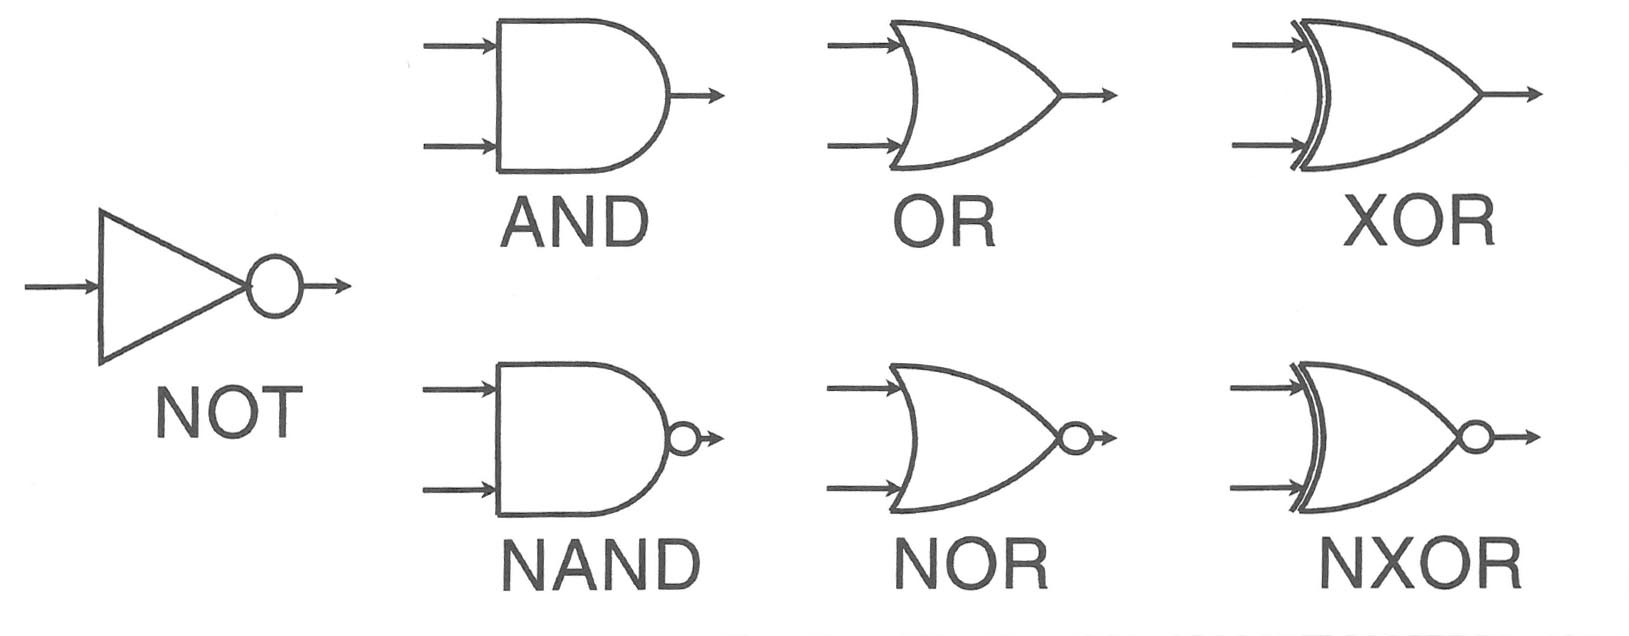
\includegraphics[width=0.9\textwidth]{SymbolesLogique.jpg}
\end{center}
\newpage
\section{Fonctions polynomiales }

Équation droite : $P(x) \equiv ax + b$ $(a,b,x \in \mathbb{R})$ \\
\tab[1cm] a : coefficient angulaire (pente) \\
\tab[1cm] b : ordonnée à l'origine

Si 2 droite on le même coefficient angulaire elles sont parallèles

Et 2 droite qui ont des coefficients angulaires opposés et inverse sont perpendiculaire\\
\tab[1cm] $y = ax + b$ et $y_\bot = \frac{-x}{a} + b$ 
\tab[.5cm] ou encore $a \cdot a_\bot = -1$

\vspace{\baselineskip}
Équation parabole : $P(x) \equiv ax^2 + bx + c$ $(a,b,c,x \in \mathbb{R})$

Factorisation de l'équation : $ax^2 + bx + c = a(x - x1)(x - x2)$ \\
\tab[1cm] Ce qui après distribution permets d'affirmer que le rapport : \\
\tab[2cm] $\frac{-b}{a}$ est égale à la somme des 2 racines : $\frac{-b}{a} = x_1 + x_2$ \\
\tab[2cm] $\frac{c}{a}$ est égale au produit des 2 racines : $\frac{c}{a} = x_1 \cdot  x_2$

\vspace{\baselineskip}
Le déterminant : $\triangle = b^2 - 4ac$ 

Permet de trouver les racines : \\
\tab[1cm] $\triangle \lt 0 $ : aucune racine réel (mais 2 racines complexes)\\
\tab[1cm] $\triangle = 0 $ : une seul racine réel (mais 2 racines complexes)\\
\tab[2cm] $x_1 = x_2 = \frac{-b}{2a}$\\
\tab[1cm] $\triangle \gt 0 $ : 2 racines réelles\\
\tab[2cm] $x_1 = \frac{-b + \sqrt{\triangle} }{2a} $
\tab[1cm] $x_2 = \frac{-b - \sqrt{\triangle} }{2a} $

\vspace{\baselineskip}
Sommet parabole : \\
\tab[1cm] x : $\frac{-b}{2a} $
\tab[1cm] y : $\frac{\triangle }{4a} $

\newpage
\section{Dérivation}

$\frac{d}{dx} c \Rightarrow 0$

$\frac{d}{dx} x \Rightarrow 1$

$\frac{d}{dx} x^n \Rightarrow nx^{n-1}$

$\frac{d}{dx} \sin(x)  \Rightarrow \cos(x)$

$\frac{d}{dx} \cos(x)  \Rightarrow -\sin(x)$

$\frac{d}{dx} \tan(x)  \Rightarrow \frac{1}{\cos^2x}$ ou $1-\tan^2(x)$

$\frac{d}{dx}  cot x \Rightarrow \frac{-1}{sin^2 x}$ ou $-(1+cot^2 x)$

$\frac{d}{dx} (f(x)\pm g(x)) \Rightarrow \frac{d}{dx} f(x) \pm \frac{d}{dx} g(x)$

$\frac{d}{dx} (f(x)\cdot  g(x)) \Rightarrow \frac{d}{dx} f(x) \cdot g(x) + f(x) \cdot \frac{d}{dx} g(x)$

$\frac{\frac{d}{dx} f(x)}{\frac{d}{dx} g(x)} \Rightarrow \frac{\frac{d}{dx} f(x)\cdot g(x)-f(x)\cdot \frac{d}{dx} g(x)}{g^2}$

$\frac{d}{dx}(c \cdot f(x)) \Rightarrow c \cdot \frac{d}{dx} f(x)$

$\frac{d}{dx} (g(x) \cdot f(x)) \Rightarrow \frac{d}{dx} g(x) \cdot (f(x) \cdot \frac{d}{dx} f(x))$

$\frac{d}{dx} \ln x \Rightarrow \frac{1}{x}$

$\frac{d}{dx} \ln (f(x)) \Rightarrow \frac{\frac{d}{dx} f(x)}{f(x)}$

$\frac{d}{dx} e^{x} \Rightarrow e^{x}$

$\frac{d}{dx} a^{x} \Rightarrow a^{x} \cdot  \ln a$

$\frac{d}{dx} \log_{a} x \Rightarrow \frac{1}{x \cdot \ln a}$

$\frac{d}{dx} \log_{a} f(x) \Rightarrow \frac{\frac{d}{dx} f(x)}{f(x) \cdot \ln a}$

$\frac{d}{dx} \sqrt{x} \Rightarrow \frac{1}{2\sqrt{x}}$

$\frac{d}{dx} \sqrt{f(x)} \Rightarrow \frac{\frac{d}{dx}}{2\sqrt{f(x)}}$

$\frac{d}{dx} \tan(f(x)) \Rightarrow \frac{\frac{d}{dx} f(x)}{\cos^2 (f(x))}$

$\frac{d}{dx}  \cot(f(x))\Rightarrow \frac{-\frac{d}{dx} f(x)}{sin^2(f(x))}$

\newpage
\section{Exponentiels et logarithmes}

$\log_a y = x \Leftrightarrow y=a^x$

$\log_a a^x = x$

$\log_b n \Rightarrow  \frac{log_a n}{log_a b}$

$\log_a \sqrt[n]{x^m} \Rightarrow \log_a x^{\frac{m}{n}} \Rightarrow \frac{m}{n} \log_a x$

$\log_a (x \cdot y) \Rightarrow \log_a x + \log_a y$

$\log_a (\frac{x}{y} ) \Rightarrow \log_a x - \log_a y$

$\log_a x^n \Rightarrow n \cdot \log_a x$

$\frac{1}{\ln a} \Rightarrow \log_a e$

$n = e^x \Rightarrow x = \log_e n \Rightarrow x = \ln n \Rightarrow n = e^{\ln n}$

\newpage
\section{Complexes}

$a + bj \Rightarrow r cjs(\theta ) \Rightarrow r \cdot e^{j\theta}$ \\
\tab[1cm]$r=\sqrt{a^2 + b^2}$ \\
\tab[1cm]$\theta = \arctan \frac{b}{a}$

$\frac{1}{a + bj} = \frac{a - bj}{a^2 - b^2}$

$\frac{1}{rcjs(\theta)} = \frac{rcjs(\theta)}{r}$

$\frac{1}{r \cdot e^{j\theta}} = \frac{e^{-j\theta}}{r}$

$\mathbb{Z}_1 \cdot \mathbb{Z}_2 = r_1 \cdot r_2 cjs(\theta_1 + \theta_2)$

$\frac{\mathbb{Z}_1}{\mathbb{Z}_2}  = \frac{r_1}{r_2} cjs(\theta_1 - \theta_2)$

$\mathbb{Z}^n = r^ncjs(n\theta)$\\
\tab[.6cm]$= r \cdot e^{jn\theta}$

\newpage
\section{Intégration}

si $\frac{d(F(x)+c)}{dx} = f(x)$, alors on dit que $F(x)$ est une primitive de $f(x)$

\Warning vu que la dérivée de $\frac{d(c)}{dx}=0$, il existe une infinité de primitive de $f(x)$ cette ensemble de primitive de $F(x)+c$ correspond à l'intégrale indéfinie de $f(x)$ et est noté $\int{f(x)dx=F(x)+c} \Leftrightarrow \frac{F(x)+c}{dx}=f(x)$  

\vspace{\baselineskip}
$\frac{d}{dx}\int{f(x)dx}=f(x)$

$\int{f(x)\pm g(x)dx}=\int{f(x)dx}\pm \int{g(x)dx}$

$\int{k f(x)dx}= k\int{f(x)dx}$

\vspace{\baselineskip}
$\int{0 dx} = c$

$\int{1 dx} = x +c$

$\int{(f(x)+g(x)) dx} = \int{f(x)dx} + \int{g(x)dx}$

$\int{\frac{f(x)dx \cdot g(x) - f(x) \cdot g(x)dx}{g(x)^2} } = \frac{f(x)}{g(x)} + c$

$\int{\frac{1}{2\sqrt{x}}dx} = \sqrt{x} +c$

$\int{\sin(x)dx} = -\cos(x)+c$

$\int{\cos(x) dx} = \sin(x)+c$

$\int{\frac{1}{\cos^2(x)} dx} = \tan(x) +c$

$\int{\frac{-1}{\sin^2(x)} dx} = \cot(x) +c$

$\int{\frac{1}{\sqrt{1-x^2} } dx} = \arcsin(x) +c$

$\int{\frac{-1}{\sqrt{1-x^2} } dx} = \arccos(x) +c$

$\int{\frac{1}{1+x^2} dx} = \arctan(x) +c$

$\int{\frac{-1}{1+x^2} dx} = \arccot(x) +c$

$\int{x^n dx} = \frac{x^{n+1}}{n+1} +c$
\tab[1cm] si n = -1 $\Rightarrow \ln \left|x\right| +c$

$\int{\frac{1}{x} dx} = \ln \left|x\right| +c$

$\int{e^x dx} = e^x+c$

$\int{a^x dx} = \frac{a^x}{\ln a} +c$

$\int{\frac{1}{x \ln a}  dx} = \log_a x +c$

$\int{f(x) dx} =\int{f(g(t)\frac{d}{dx} g(t)dt)}$\\
\tab[1.8cm]$\Rightarrow x = g(t)$

$\int{f(x) \frac{d}{dx} g(x) dx} = f(x)g(x)-\int{\frac{d}{dx} f(x)g(x) dx}$

$\int{f(x)g(x) dx} = \frac{d}{dx} f(x)g(x) + f(x)\frac{d}{dx} g(x)+c$

$\int{\frac{\frac{d}{dx} f(x)}{f(x)}  dx} = \ln \left|f(x)\right| +c$

$\int{\frac{d}{dx} f(x) e^{f(x)} dx} = e^{f(x)}+c$

$\int{\frac{d}{dx} f(x)\sin(f(x)) dx} = -\cos(f(x)) +c$

$\int{\frac{d}{dx} f(x)\cos(f(x)) dx} = \sin(f(x)) +c$

$\int{\frac{\frac{d}{dx} f(x)}{\sqrt{1-(f(x))^2} }  dx} = \arcsin(f(x)) +c$

$\int{\frac{\frac{d}{dx} f(x)}{\cos^2(f(x))}  dx} = \tan(f(x))+c$

\newpage
\section{Statistiques}

Le rôle de la statistique, c'est une aide à la prise de décision

Statistique au singulier ou statistiques au pluriel : 
\begin{itemize}%\setlength{\itemsep}{0mm}
    \item au singulier : c'est l'ensemble des méthode scientifique dont le but est de traite des données 
    \item au pluriel : ce sont les les données d'observation chiffrées 
\end{itemize}

\subsection{Concept de bases}
\begin{description}%[style=nextline]
   \item[population] l'ensemble des individu ou des objets dont une ou plusieurs caractéristiques nous intéresse 
   \item[échantillon] un sous ensemble représentatif de la population qui fournira les données à traiter
   \item[caractère de la variable] 
        \begin{itemize}%\setlength{\itemsep}{0mm}
            \item variable qualitative : c'est à dire non numérique (sexe, ...)
            \item variable quantitative : c'est à dire numérique (taille, ...)
        \end{itemize}
   \item[Vaiable quantitative] peuvent être soit discrète, c'est à dire un ensemble fini de valeurs, soit continu c'est à dire un ensemble des valeurs prenant toutes les valeurs possible de l'ensemble
   \item[série] 
        \begin{itemize}%\setlength{\itemsep}{0mm}
            \item statistique qui est constituer d'un ensemble de valeurs prise par une variable à un moment donné
            \item  chronologique qui est constituer d'un ensemble d'une valeur prise sur un temps
        \end{itemize}
\end{description}

\subsection{Mise en classe}
\begin{description}%[style=nextline]
   \item[Nombre de classe] K : $1 + \frac{10}{3} \log n$
    \tab[1cm] n : taille de l'échantillon \\
     \Warning Toujours arrondir à l'unité supérieur
   \item[Étendue] E : $X_{max} - X_{min}$
   \item[Longueur de classe] l : $\frac{E}{K}$ \\
    \Warning Toujours arrondir à l'unité supérieur
   \item[Excédant] Exc : $K\cdot l -E$
   \begin{itemize}%\setlength{\itemsep}{0mm}
         \item Borne inférieur $X_{min} - Exc$
         \item Borne supérieur $X_{max} + Exc$
    \end{itemize}
   \item[Centre de classe] $X_{centj}$ \tab[1cm] j = indice de la classe
   \item[Effectif simple] nombre de valeur contenue dans la classe nj
   \item[Effectif cumulé] nombre de valeur contenue dans la classe $+$ la précédente (cumulée) Nj 
   \item[Fréquence simple] fj : $\frac{nj}{n}\cdot 100 \%$
   \item[Fréquence cumulée] fréquence de la classe $+$ la précédente (cumulée) Fj 
\end{description}

\subsection{Paramètres d'étendue}
\begin{description}%[style=nextline]
   \item[Moyenne arithmétique] MA : valeur moyenne $\frac{1}{n} \sum\limits_{j=1}^{k}{n_j \cdot X_{centj}}$
   \item[Médiane] ME : $X_{centj} + l(\frac{\frac{n}{2} - N_{j^*-1}}{n_{j^*}})$ \tab[1cm] j* indice de la classe dont la fréquence est directement $\geq$ 50\%
   \item[Mode] MO : valeur la plus souvent observée 3ME - 2MA
   \item[Variance] $S^2$ $\frac{1}{n}\sum\limits_{j=1}^{K}{n_j(X_{centj}-MA)^2}  $
   \item[Écart type] S : $\sqrt{S^2}$ 
    \begin{itemize}%\setlength{\itemsep}{0mm}
            \item MA - S $\rightarrow$ MA + S$\Rightarrow$ 67\%
            \item MA - 2S $\rightarrow$ MA +2S $\Rightarrow$ 95\%
            \item MA - 3S $\rightarrow$ MA + 3S $\Rightarrow$ 99\%
        \end{itemize}
   \item[Intervalle inter-quartile]
        \begin{itemize}%\setlength{\itemsep}{0mm} 
            \item $Q_1$ : $X_{minj^*}+l(\frac{\frac{n}{4} -N_{j^*-1}}{n_{j^*}})$ \tab[1cm] j* indice de la classe dont la fréquence est directement $\geq$ 25\%
            \item  $Q_3$ : $X_{minj^*}+l(\frac{\frac{3n}{4} -N_{j^*-1}}{n_{j^*}})$ \tab[1cm] j* indice de la classe dont la fréquence est directement $\geq$ 75\%
        \end{itemize}
    \item[Coefficient de Pearson] $S_K$ : $\frac{MA - MO}{S}$
    \item[Coefficient de Yule \& Kendal] $Y_K$ : $\frac{(Q_3 - ME)-(ME-Q_1)}{Q_3-Q_1}$ \\
        \tab[2cm] \Warning toujours $-1\leq Y_K\leq 1 $
\end{description}
\end{document}
